We restrict ourselves to feed-forward sequential NNs where only the parameters of the linear layers are trainable.
To derive a Kronecker-factored approximation of the Gramian, we first describe how a layer's parameter enters the Laplacian's computation in~\Cref{sec:laplacian-computation-graph}.
This allows for expressing the exact Gramian as a sum over Kronecker-structured terms stemming from the parameter's direct children in the compute graph, see~\Cref{sec:kronecker-structure-gramian}.

\subsection{Hessian Backpropagation}\label{sec:laplacian-computation-graph}
Here we derive the Laplacian of a feed-forward neural network with scalar output, that is $\Delta u_{\vtheta} := \Tr(\gradsquared{\vx} u_{\theta})$.
The goal is to make the dependence of the Laplacian w.r.t.\,a weight $\mW$ in one layer of the network explicit.
Then we can write down the Jacobian $\jac_{\mW}(\Delta u_{\vtheta})$ which is required for the Fisher used by energy NGD.

We first lay out the notation for feedforward neural networks, then use the ideas of Hessian backpropagation \citep[HBP,][]{dangel2020modular} to derive a recursion for the Hessian $\gradsquared{\vx}u_{\vtheta}$.
The Laplacian follows by taking the trace of the latter.
Finally, we express the Laplacians gradient w.r.t.
a single layer's weight $\mW$, i.e.\,$\nicefrac{\partial \Delta u_{\vtheta}}{\partial \mW}$, in terms of $\mW$'s children in the compute graph.

\subsection{Feed-forward Neural Networks}
\paragraph{Layer notation} Consider a sequential neural network $u_{\vtheta}$ with depth $L$ that consists of layers $f^{(i)}_{\vtheta^{(i)}}$ with trainable parameters $\vtheta^{(i)} \in \sR^{d^{(i)}}, i=1,\dots, L,$ that transform an input $\vx \in \sR^M$ into a prediction $u_{\vtheta}(\vx)\in \sR^C$ via intermediate representations $\vz^{(i)} \in \sR^{h^{(i)}}, i= 0, \dots, L$,
\begin{align}
  \begin{split}
    u_{\vtheta}
    &=
      f^{(L)}_{\vtheta^{(L)}} \circ f^{(L-1)}_{\vtheta^{(L-1)}} \circ \ldots \circ f^{(1)}_{\vtheta^{(1)}}
    \\
    f^{(i)}_{\vtheta^{(i)}}: \sR^{h^{(i-1)}}
    &\to
      \sR^{h^{(i)}}\,,
    \\
    \vz^{(i-1)}
    &\mapsto
      \vz^{(i)} = f^{(i)}_{\vtheta^{(i)}}(\vz^{(i-1)})
  \end{split}
\end{align}
where $\vz^{(0)} := \vx$, $\vz^{(L)} := \vu$, and $\vtheta = ({\vtheta^{(1)}}^{\top}, \dots, {\vtheta^{(L)}}^{\top})^{\top}$ is the concatenation of parameters over layers.
A parameter might be empty, e.g.\,if the layer is an activation layer.

\subsection{Derivatives}

\paragraph{Flattening} Above, we assumed all quantities ($\vz^{(i)}, \vtheta^{(i)}$) to be vectors.
In case of tensor-valued quantities, we can first flatten them into vectors to reduce to the vector case.
Our index convention to vectorize will be first-varies-fastest, which means column-stacking for a matrix (row index varies first, column index varies second).
We denote the flattening operation by $\flatten(\cdot)$.

\paragraph{Jacobian \& Hessian} The flattening notation allows to reduce derivatives of matrix/tensor-valued objects back to the matrix case.
Consider the Jacobian $\jac_{\va}\vb$ of a vector $\vb$ w.r.t.\,a vector $\va$.
It collects all partial derivatives as $[\mJ_{\va}\vb]_{i,j} = \nicefrac{\partial [\vb]_i}{\partial [\va]_j}$.
For the Jacobian $\jac_{\mA}\mB$ of a matrix $\mB$ w.r.t.\,a matrix $\mA$, we simply have $\jac_{\mA} \mB = \jac_{\flatten( \mA )}\flatten(\mB)$.
Likewise, the Hessian $\gradsquared{\va}b$ of a scalar $b$ w.r.t.\,a vector $\va$ collects the second-order partial derivatives according to $[\gradsquared{\va}b]_{i,j} = \nicefrac{\partial^2 b}{\partial [\va]_i \partial [\va]_j}$.
For the Hessian $\gradsquared{\mA} b$ of a scalar $b$ w.r.t.\,a matrix $\mA$, we simply have $\gradsquared{\mA} b = \gradsquared{\flatten(\mA)}b$.
We also have $\grad{\mA} b = \grad{\flatten(\mA)} b$ for the gradient of a scalar w.r.t.\,a matrix.

\subsection{Input Hessian}

Gradient backpropagation describes a recursive procedure to compute gradients by backpropagating a signal via vector-Jacobian products (VJPs).
A similar procedure can be derived to compute Hessians w.r.t.\,nodes in a graph ($\vz^{(i)}$ or $\vtheta^{(i)}$).
We call this recursive procedure Hessian backpropagation~\citep{dangel2020modular}.

In the following, we set $C = 1$, that is the neural network produces a scalar $u$.

\paragraph{Gradient backpropagation} As a warm-up, let's recall how to compute the gradient $\grad{\vtheta}u =
(\grad{\vtheta^{(1)}} \dots \grad{\vtheta^{(L)}})$. We start by setting $\grad{u}
u = 1$, then backpropagate the error via VJPs,
\begin{align}\label{eq:gradient-backpropagation}
  \begin{split}
    \grad{\vz^{(i-1)}}u
    &=
      \left( \jac_{\vz^{(i-1)}} \vz^{(i)} \right)^{\top} \grad{\vz^{(i)}}u\,,
    \\
    \grad{\vtheta^{(i)}}u
    &=
      \left( \jac_{\vtheta^{(i)}} \vz^{(i)} \right)^{\top} \grad{\vz^{(i)}}u\,
  \end{split}
\end{align}
for $i = L, \dots, 1$, and initialization $\grad{\vz^{(L)}}u = \grad{u}u = 1$ of the recursion.
This yields the gradients of $u$ w.r.t.\,all intermediate representations and parameters.

\paragraph{Hessian backpropagation} The recursion for computing Hessians of $u$
w.r.t.\,intermediate representations and parameters starts by initializing the
recursion with $\gradsquared{\vz^{(L)}}u = \gradsquared{u} u = 0$, then
backpropagates according to
\begin{align}\label{eq:hessian-backpropagation}
  \begin{split}
    \gradsquared{\vz^{(i-1)}}u
    &=
      \left( \jac_{\vz^{(i-1)}} \vz^{(i)} \right)^{\top}
      \gradsquared{\vz^{(i)}}u
      \left( \jac_{\vz^{(i-1)}} \vz^{(i)} \right)
      +
      \sum_{k=1}^{h^{(i)}}
      \left(
      \gradsquared{\vz^{(i-1)}} [\vz^{(i)}]_k
      \right)
      [\grad{\vz^{(i)}} u]_k\,,
    \\
    \gradsquared{\vtheta^{(i)}}u
    &=
      \left( \jac_{\vtheta^{(i)}} \vz^{(i)} \right)^{\top}
      \gradsquared{\vz^{(i)}}u
      \left( \jac_{\vtheta^{(i)}} \vz^{(i)} \right)
      +
      \sum_{k=1}^{h^{(i)}}
      \left(
      \gradsquared{\vtheta^{(i)}} [\vz^{(i)}]_k
      \right)
      [\grad{\vz^{(i)}} u]_k
  \end{split}
\end{align}
for $i = L, \dots, 1$.
The first term takes the incoming Hessian (w.r.t.\,a layer's output) and sandwiches it between the layer's Jacobian.
It can be seen as backpropagating curvature from downstream layers.
The second term adds in curvature introduced by the current layer.
It is only non-zero if the layer is non-linear.
For linear layers, convolutional layers, and ReLU layers, it is zero.

\begin{figure}[t]
  \centering
  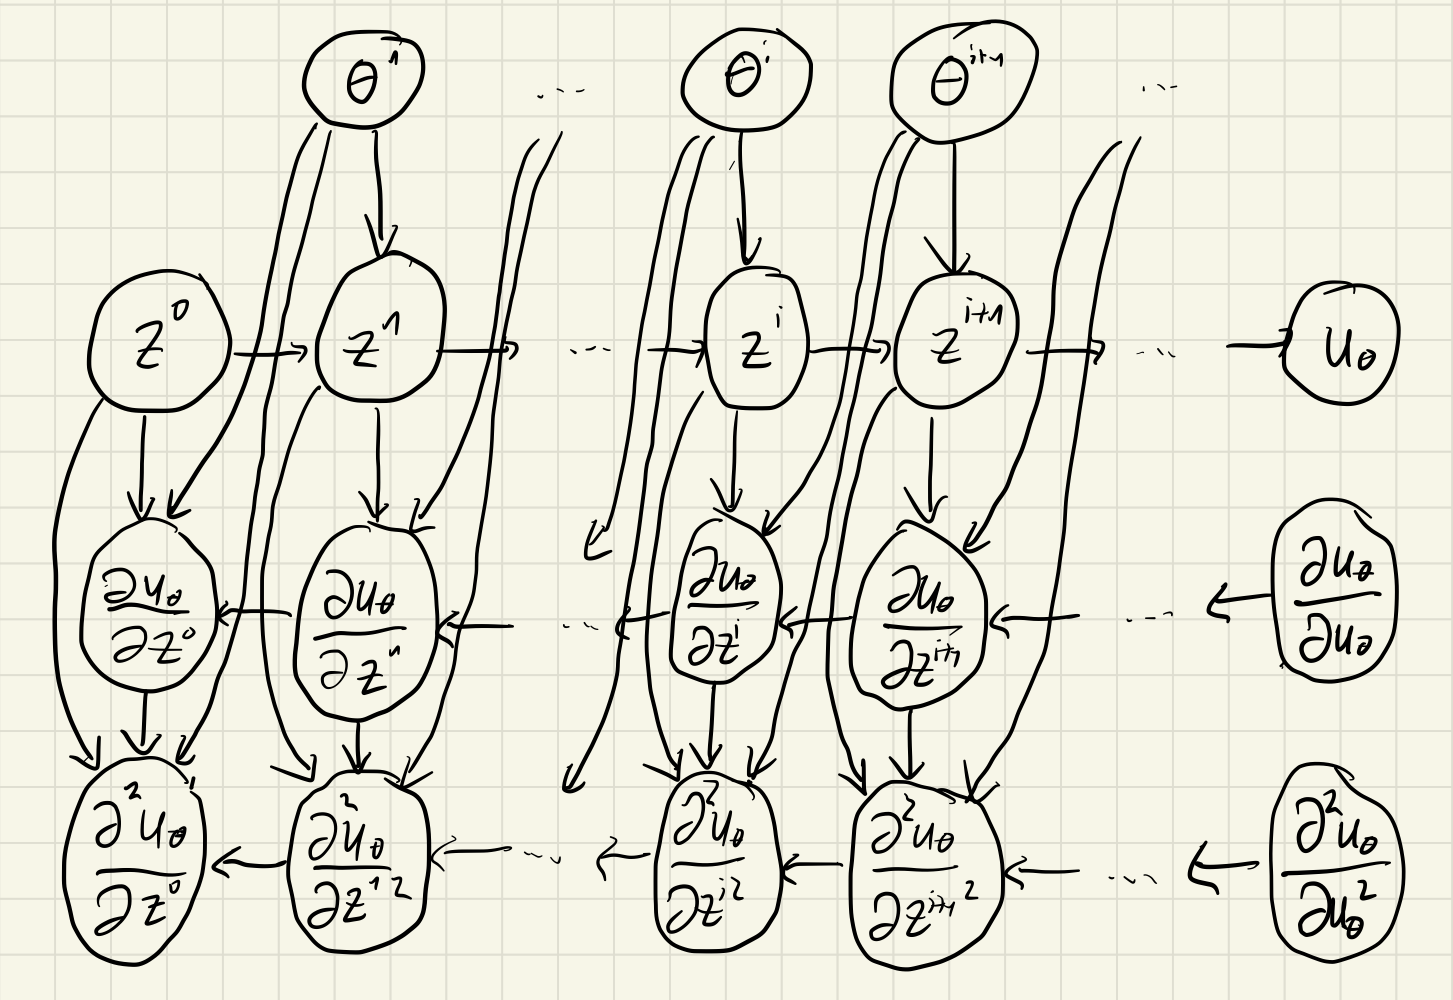
\includegraphics[width=0.6\linewidth]{figures/HBP_graph.png}
  \caption{Dependencies during gradient and Hessian backpropagation when computing the Hessian $\gradsquared{\vx}u_{\vtheta}$.}\label{fig:hbp-dependencies}
  \label{fig:hbp-dependencies}
\end{figure}

Following the procedure of \Cref{eq:hessian-backpropagation} yields the
per-layer parameter and feature Hessians $\gradsquared{\vz^{(i)}}u,
\gradsquared{\vtheta^{(i)}}u$. In \Cref{fig:hbp-dependencies} we depict the dependencies of
intermediate gradients and Hessians for computing $\gradsquared{\vx}u_{\vtheta}$:
\begin{itemize}
\item $\grad{\vz^{(i-1)}}u$ depends on $\grad{\vz^{(i)}}$ due to the recursion in \Cref{eq:gradient-backpropagation}, and on $\vz^{(i-1)}, \vtheta^{(i)}$ due to the Jacobian $\mJ_{\vz^{(i-1)}}\vz^{(i)}$ in the gradient backpropagation \Cref{eq:gradient-backpropagation}.

\item $\gradsquared{\vz^{(i-1)}}u$ depends on $\gradsquared{\vz^{(i)}}u$ and $\grad{\vz^{(i)}} u$ due to the recursion in \Cref{eq:hessian-backpropagation}, and on $\vz^{(i-1)}, \vtheta^{(i)}$ due to the Jacobian $\mJ_{\vz^{(i-1)}}\vz^{(i)}$ and Hessian $\gradsquared{\vz^{(i-1)}}[\vz^{(i)}]_k$ in the Hessian backpropagation \Cref{eq:gradient-backpropagation}.
\end{itemize}

\subsection{Laplacian}

The Laplacian $\Delta u_{\vtheta}$ follows by taking the trace of
$\gradsquared{\vx}u_{\vtheta}$ from above, and is hence recursively defined.

\begin{figure}[t]
  \centering
  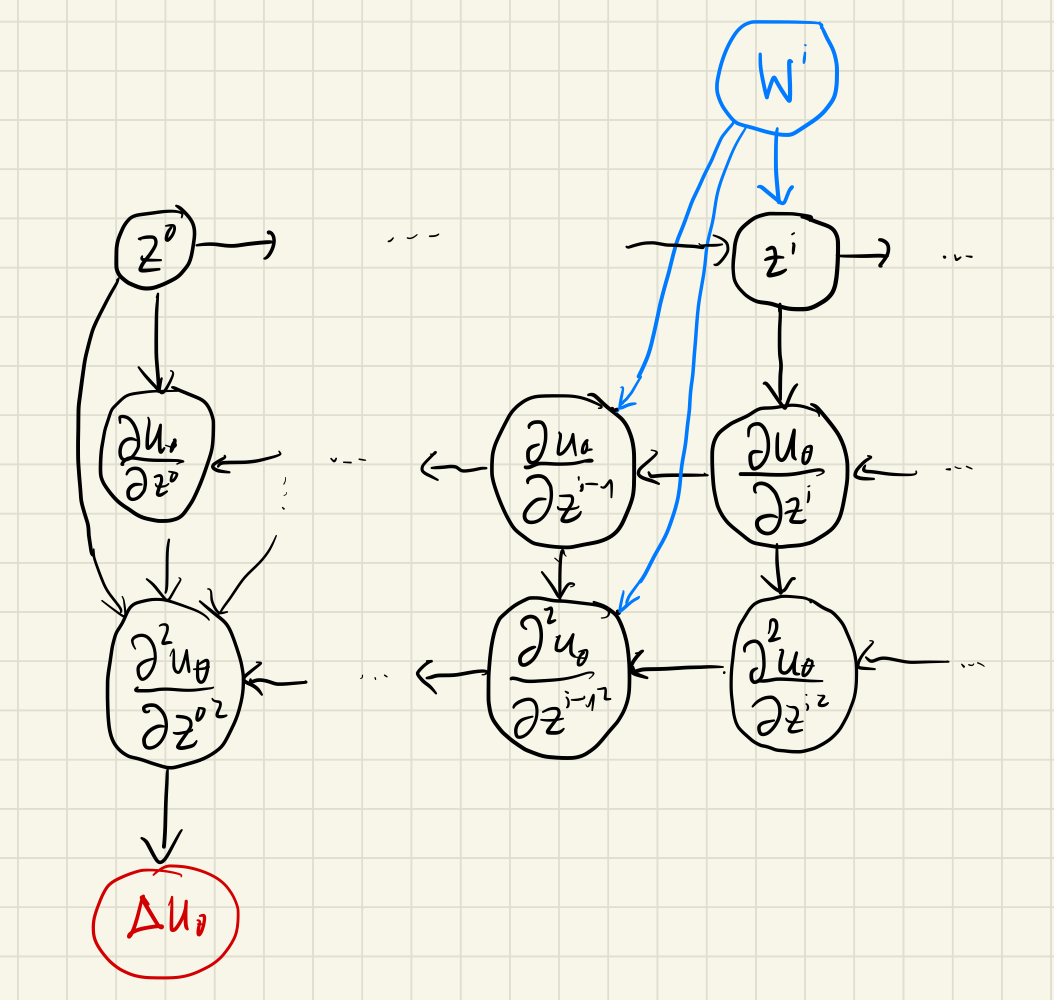
\includegraphics[width=0.6\linewidth]{figures/HBP_graph_weight.png}
  \caption{Direct children of the weight matrix of a single layer for the computation graph of the Laplacian.}\label{fig:laplacian-graph-weight}
\end{figure}

\paragraph{For a linear layer} To de-clutter the dependency graph of \Cref{fig:hbp-dependencies}, we will now consider the dependency of $\Delta u_{\vtheta}$ w.r.t.\,the weight of a single layer.
We assume this layer $i$ to be a linear layer with parameters $\mW^{(i)}$ such that $\vtheta^{(i)} = \flatten(\mW^{(i)})$,
\begin{align}
  \vz^{(i)} = \mW^{(i)} \vz^{(i-1)}\,.
\end{align}
For this layer, the second terms in \Cref{eq:hessian-backpropagation} disappears because the local Hessians are zero, that is $\gradsquared{\vz^{(i-1)}}[\vz^{(i)}]_k = \vzero$ and $\gradsquared{\mW^{(i)}}[\vz^{(i)}]_k = \vzero$.
Also, the Jacobians are $\jac_{\mW^{(i)}}\vz^{(i)} = {\vz^{(i-1)}}^{\top} \otimes \mI$ and $\jac_{\vz^{(i-1)}}\vz^{(i)} = \mW^{(i)}$ and hence only depends on one of the two layer inputs.
This simplifies the computation graph.
\Cref{fig:laplacian-graph-weight} shows the dependencies of $\mW^{(i)}$ on the
Laplacian, highlighting its three direct children,
\begin{align}
  \begin{split}
    \vz^{(i)}
    &=
      \mW^{(i)} \vz^{(i-1)}
    \\
    \grad{\vz^{(i-1)}}u
    &=
      {\mW^{(i)}}^{\top}
      \left(
      \grad{\vz^{(i)}}u
      \right)
    \\
    \gradsquared{\vz^{(i-1)}}u
    &=
      {\mW^{(i)}}^{\top}
      \left(
      \gradsquared{\vz^{(i)}}u
      \right)
      \mW^{(i)}
  \end{split}
\end{align}

\paragraph{Laplacian's derivative for a linear layer} We have now identified the direct children of $\mW^{(i)}$ in the Laplacian's compute graph.
This allows us to write down its derivative $\grad{\mW^{(i)}} \Delta u$, which---by the chain rule---is simply the accumulated backpropagated error from the direct children:
\begin{align}\label{eq:laplacian-gradient}
  \begin{split}
    \grad{\mW^{(i)}} \Delta u_{\vtheta}
    &=
      \sum_{\bullet \in \left\{ \vz^{(i)}, \grad{\vz^{(i-1)}}u, \gradsquared{\vz^{(i-1)}}u \right\}}
      \left(
      \jac_{\mW^{(i)}}\bullet
      \right)^{\top}
      \grad{\bullet}\Delta u
    \\
    &=
      \left(
      \jac_{\mW^{(i)}}\vz^{(i)}
      \right)^{\top}
      \grad{\vz^{(i)}}\Delta u
      +
      \left(
      \jac_{\mW^{(i)}}\grad{\vz^{(i)}}u
      \right)^{\top}
      \grad{\grad{\vz^{(i)}}u}\Delta u
      +
      \left(
      \jac_{\mW^{(i)}}\gradsquared{\vz^{(i)}}u
      \right)^{\top}
      \grad{\gradsquared{\vz^{(i)}}u}\Delta u\,.
  \end{split}
\end{align}

\paragraph{The Fisher} With the Laplacian's gradient \Cref{eq:laplacian-gradient}, we can write down the Fisher block for $\mW^{(i)}$
\begin{align}\label{eq:fisher}
  \begin{split}
    \mF^{(i)}
    &=
      \left(
      \grad{\mW^{(i)}} \Delta u_{\vtheta}
      \right)
      \left(
      \grad{\mW^{(i)}} \Delta u_{\vtheta}
      \right)^{\top}
    \\
    &=
      \sum_{\textcolor{blue}{\bullet} \in \left\{ \vz^{(i)}, \grad{\vz^{(i-1)}}u, \gradsquared{\vz^{(i-1)}}u \right\}}
      \sum_{\textcolor{red}{\bullet} \in \left\{ \vz^{(i)}, \grad{\vz^{(i-1)}}u, \gradsquared{\vz^{(i-1)}}u \right\}}
      \left(
      \left(
      \jac_{\mW^{(i)}}\textcolor{blue}{\bullet}
      \right)^{\top}
      \grad{\textcolor{blue}{\bullet}}\Delta u
      \right)
      \left(
      \left(
      \jac_{\mW^{(i)}}\textcolor{red}{\bullet}
      \right)^{\top}
      \grad{\textcolor{red}{\bullet}}\Delta u
      \right)^{\top}
    \\
    &=
      \sum_{\textcolor{blue}{\bullet} \in \left\{ \vz^{(i)}, \grad{\vz^{(i-1)}}u, \gradsquared{\vz^{(i-1)}}u \right\}}
      \sum_{\textcolor{red}{\bullet} \in \left\{ \vz^{(i)}, \grad{\vz^{(i-1)}}u, \gradsquared{\vz^{(i-1)}}u \right\}}
      \underbrace{
      \left(
      \jac_{\mW^{(i)}}\textcolor{blue}{\bullet}
      \right)^{\top}
      \left[
      \left(
      \grad{\textcolor{blue}{\bullet}}\Delta u
      \right)
      \left(
      \grad{\textcolor{red}{\bullet}}\Delta u
      \right)^{\top}
      \right]
      \left(
      \jac_{\mW^{(i)}}\textcolor{red}{\bullet}
      \right)}_{
      := \mF^{(i)}_{\textcolor{blue}{\bullet}, \textcolor{red}{\bullet}}
      }\,.
  \end{split}
\end{align}
The Fisher consists of nine different terms.
Eventually, we would like to approximate it with a single Kronecker product, like KFAC~\citep{martens2015optimizing}.
Note that one of the nine terms is the term from the original KFAC paper, namely
when $\textcolor{blue}{\bullet} = \textcolor{red}{\bullet} = \vz^{(i)}$
(remember that $\jac_{\mW^{(i)}} \vz^{(i)} = \vz^{(i-1)} \otimes \mI$):
\begin{align}\label{eq:original-kfac}
  \begin{split}
    \mF^{(i)}_{\textcolor{blue}{\vz^{(i)}}, \textcolor{red}{\vz^{(i)}}}
    &=
      \left(
      \textcolor{blue}{\vz^{(i-1)} \otimes \mI}
      \right)
      \left[
      \left(
      \textcolor{blue}{\grad{\vz^{(i-1)}}\Delta u}
      \right)
      \left(
      \textcolor{red}{\grad{\vz^{(i-1)}}\Delta u}
      \right)^{\top}
      \right]
      \left(
      \textcolor{red}{{\vz^{(i-1)}}^{\top} \otimes \mI}
      \right)
    \\
    &=
      \textcolor{blue}{\vz^{(i-1)}}
      \textcolor{red}{{\vz^{(i-1)}}^{\top}}
      \otimes
      \left(
      \textcolor{blue}{\grad{\vz^{(i-1)}}\Delta u}
      \right)
      \left(
      \textcolor{red}{\grad{\vz^{(i-1)}}\Delta u}
      \right)^{\top}
    \\
    &:= \mA_{\text{KFAC}}^{(i)} \otimes \mB_{\text{KFAC}}^{(i)}\,.
  \end{split}
\end{align}
\Cref{eq:original-kfac} illustrates that the Kronecker structure emerges from
the Jacobians. So we need to investigate these objects closer for the remaining
terms of \Cref{eq:fisher}.

\paragraph{Jacobians from the gradient and Hessian backward pass} We already know the Jacobian from the linear layer's forward pass,
\begin{subequations}\label{eq:fisher-jacobians}
  \begin{align}
    \jac_{\mW}\left( \mW \vx \right) = \vx^{\top} \otimes \mI\,.
  \end{align}
  The Jacobian from the gradient backpropagation is
  \begin{align}
    \jac_{\mW}\left( \mW^{\top} \vx \right) = \mI \otimes \vx^{\top}\,,
  \end{align}
  and the Jacobian from the Hessian backpropagation is
  \begin{align}
    \jac_{\mW}\left( \mW^{\top} \mX \mW \right) = \mI \otimes \mW^{\top}\mX + \mI \otimes \mW^{\top}\mX^{\top}\,.
  \end{align}
\end{subequations}
\toodoo{F.D.\,derived the Jacobians from \Cref{eq:fisher-jacobians} by hand.
  Might be worth to double-check for correctness.}
The Jacobians from \Cref{eq:fisher-jacobians} allow to express the Fisher in
terms of Kronecker-structured expressions consisting of 16 terms in total.

\toodoo{F.D.\,Write down the full expression for the Fisher.
  Propose ways to Kronecker-approximate each of the 16 terms, such that we end up with a single Kronecker product in the end.}

%%% Local Variables:
%%% mode: latex
%%% TeX-master: "../main"
%%% End:


\subsection{Kronecker Structure of the Gramian}\label{sec:kronecker-structure-gramian}

This subsection describes the Jacobians of the operations with the weight matrix in
a linear layer during the computation of the Laplacian and ends by providing an
equation for the Gramian block.

\subsection{Kronecker-factored Approximate Gramian (KFAG)}
This subsection describes the Kronecker approximation we propose for the per-layer Gramian.
It should also justify that the approximation is similar to that in other works.

\toodoo{F.D.
  Warning: The below write-up is a first attempt to come up with a Kronecker approximation.
  I still need to find more intuitive explanations, ideally with ideas from other KFAC papers.}

We will rely on a similar intuition than \citet{eschenhagen2023kroneckerfactored} in the presence of weight sharing.
However, we will use a slightly different motivation to obtain the Kronecker structure in the presence of weight sharing.

\paragraph{Some intuition:} Consider a weight matrix $\mW \in \sR^{D_1 \times
  D_2}$ inside a neural network that produces a loss $\ell$. We want to compute
the Gramian $\mF(\mW) = \grad{\mW}\ell (\grad{\mW}\ell)^{\top}$. Consider the following scenarios:
\begin{enumerate}
\item \textbf{(No sharing, no transpose)} The matrix is used to form the matrix vector product $\vz = \mW \vx \in \sR^{D_2}$ with an input vector $\vx \in \sR^{D_1}$.
  The Gramian is then
  \begin{align*}
    \mF(\mW) = \vx \vx^{\top} \otimes \grad{\vz}\ell (\grad{\vz}\ell)^{\top}\,.
  \end{align*}
  The input to the matrix multiply forms the first Kronecker factor, the gradient w.r.t.\,the matrix multiply's output forms the second Kronecker factor.

\item \textbf{(No sharing, transpose)} The matrix is used to form the transpose matrix vector product $\vz = \mW^{\top} \vx \in \sR^{D_1}$.
  The Gramian is then
  \begin{align*}
    \mF(\mW) = \grad{\vz}\ell (\grad{\vz}\ell)^{\top} \otimes \vx \vx^{\top}\,.
  \end{align*}
  The gradient w.r.t.\,the transpose matrix multiply's output forms the first Kronecker factor, the input to the matrix multiply forms the second Kronecker factor.
  I.e.
  the Gramian w.r.t.\,the transpose matrix is just the Gramian of the non-transposed matrix, but with swapped Kronecker factors.

\item \textbf{(Sharing, no transpose)} The matrix is used to form the matrix matrix product $\mZ = \mW \mX \in \sR^{D_2 \times S}$ with an input matrix $\mX \in \sR^{D_1 \times S}$ consisting of $S$ vector-valued columns which share the same weights.
  The Gramian is then
  \begin{align*}
    \mF(\mW) =
    \left(
    \mX
    \otimes
    \mI_{D_2}
    \right)
    \grad{\mZ}\ell (\grad{\mZ}\ell)^{\top}
    \left(
    \mX^{\top}
    \otimes
    \mI_{D_2}
    \right)
  \end{align*}
  Note that this does not simplify into a single Kronecker product.
  We need to apply another approximation.
  One way to obtain a single Kronecker factor is to seek an approximation for the central term such that $\grad{\mZ}\ell (\grad{\mZ}\ell)^{\top} \approx \mI \otimes \mU$ with $\mU \in \sR^{D_1 \times D_1}$.
  Let's look for the matrix that minimizes the reconstruction error
  $\left\lVert \grad{\mZ}\ell (\grad{\mZ}\ell)^{\top} - \mI \otimes \mU
  \right\rVert_{\text{F}}^2$. The solution to this is given by the average
  diagonal blocks of $\grad{\mZ}\ell (\grad{\mZ}\ell)^{\top}$. We can write it
  as
  \begin{align}
    \mU
    =
    \frac{1}{S}
    \flatten^{-1}
    \left(
    \grad{\mZ}\ell
    \right)
    \left[
    \flatten^{-1}
    \left(
    \grad{\mZ}\ell
    \right)
    \right]^{\top}
  \end{align}
  where $\flatten^{-1} \left(\grad{\mZ}\ell \right) \in \sR^{D_1 \times S}$.
  With this approximation, we can express the Gramian as a single Kronecker product:
  \begin{align*}
    \begin{split}
      \mF(\mW)
      &\approx
        \left(
        \mX
        \otimes
        \mI_{D_2}
        \right)
        \left(
        \mI
        \otimes
        \mU
        \right)
        \left(
        \mX^{\top}
        \otimes
        \mI_{D_2}
        \right)
      \\
      &=
        \mX \mX^{\top}
        \otimes
        \mU
      \\
      &=
        \mX \mX^{\top}
        \otimes
        \frac{1}{S}
        \flatten^{-1}
        \left(
        \grad{\mZ}\ell
        \right)
        \left[
        \flatten^{-1}
        \left(
        \grad{\mZ}\ell
        \right)
        \right]^{\top}
    \end{split}
  \end{align*}
  Again, note that the input to the matrix multiply forms the first Kronecker factor, the gradient w.r.t.\,the matrix multiply's output forms the second Kronecker factor.
  However, we needed additional approximations to obtain a single Kronecker product.

\item \textbf{(Sharing, transpose)} The matrix is used to form the transpose matrix matrix product $\mZ = \mW^{\top} \mX \in \sR^{D_1 \times S}$ with $\mX \in \sR^{D_2 \times S}$.
  The Gramian is then
  \begin{align*}
    \begin{split}
      \mF(\mW)
      &=
        \left(
        \mI_{D_1}
        \otimes
        \mX
        \right)
        \mK^{\top}
        \grad{\mZ}\ell (\grad{\mZ}\ell)^{\top}
        \mK
        \left(
        \mI_{D_1}
        \otimes
        \mX^{\top}
        \right)\,.
    \end{split}
  \end{align*}
  Again, this does not simplify into a single Kronecker product.
  So we are forced to make another approximation.
  Let's first take a closer look at $\mK^{\top} \grad{\mZ}\ell$.
  The application of $\mK^{\top}$ simply changes the flattening scheme of the vector.
  With the definition $\grad{\mZ^{\top}}\ell := \grad{\flatten(\mZ^{\top})} \ell$, we have that $\mK^{\top} \grad{\mZ}\ell = \grad{\mZ^{\top}}\ell$.
  Just like in the (sharing, no transpose) case from above, we will now look for an approximation of $\grad{\mZ^{\top}}\ell (\grad{\mZ^{\top}}\ell)^{\top} \approx \mU \otimes \mI$ with $\mU \in \sR^{D_1\times D_1}$.
  Again, we choose $\mU$ to minimize the reconstruction $\left\lVert \grad{\mZ^{\top}}\ell (\grad{\mZ^{\top}}\ell)^{\top} - \mU \otimes \mI \right\rVert_{\text{F}}^2$.
  We can transform this by applying $\mK$ from the left and from the right before evaluating the squared Frobenius norm (this only rearranges the elements and the Frobenius norm does not depend on the order).
  So we have $\left\lVert \mK \left( \grad{\mZ^{\top}}\ell (\grad{\mZ^{\top}}\ell)^{\top} - \mU \otimes \mI \right) \mK \right\rVert_{\text{F}}^2 = \left\lVert \grad{\mZ}\ell (\grad{\mZ}\ell)^{\top} - \mI \otimes \mU \right\rVert_{\text{F}}^2 $, which is the same objective from the (sharing, no transpose) case.
  Hence, its solution is $\mU = \nicefrac{1}{S} \flatten^{-1}
  \left(\grad{\mZ}\ell \right) \left[\flatten^{-1} \left(\grad{\mZ}\ell \right)
  \right]^{\top}$. With that, the single Kronecker product approximation of the
  Fisher is
  \begin{align*}
    \begin{split}
      \mF^{(i)}
      &\approx
        \left(
        \mI_{D_1}
        \otimes
        \mX
        \right)
        \left(
        \mU
        \otimes
        \mI_{S}
        \right)
        \left(
        \mI_{D_1}
        \otimes
        \mX^{\top}
        \right)
      \\
      &=
        \mU
        \otimes
        \mX \mX^{\top}
      \\
      &=
        \frac{1}{S}
        \flatten^{-1}
        \left(
        \grad{\mZ}\ell
        \right)
        \left[
        \flatten^{-1}
        \left(
        \grad{\mZ}\ell
        \right)
        \right]^{\top}
        \otimes
        \mX \mX^{\top}
    \end{split}
  \end{align*}
  The input to the transpose matrix multiply forms the first Kronecker factor, the gradient w.r.t.\,the transpose matrix multiply's output forms the second Kronecker factor.

\end{enumerate}

\paragraph{Single datum case} As a first step, let's write down only the diagonal terms of the Gramian, i.e.\,the terms caused by the same children and try to simplify each term into a Kronecker product of same dimension:
\begin{align}
  \begin{split}
    \mF^{(i)}
    &\approx
      \underbrace{
      \left(
      {\vz^{(i-1)}}^\top\otimes \mI
      \right)^{\top}
      \grad{\vz^{(i)}}\Delta u
      \left(
      \left(
      {\vz^{(i-1)}}^\top\otimes \mI
      \right)^{\top}
      \grad{\vz^{(i)}}\Delta u
      \right)^{\top}
      }_{(1, 1)}
    \\
    &\phantom{=}+
      \underbrace{
      \left(
      \mI \otimes \grad{\vz^{(i)}}u
      \right)^{\top}
      \grad{\grad{\vz^{(i-1)}}u}\Delta u
      \left(
      \left(
      \mI \otimes \grad{\vz^{(i)}}u
      \right)^{\top}
      \grad{\grad{\vz^{(i-1)}}u}\Delta u
      \right)^{\top}
      }_{(2, 2)}
    \\
    &\phantom{=}+
      \underbrace{
      2
      \left(
      \mI \otimes
      \left[
      \left( \gradsquared{\vz^{(i)}}u \right) \mW^{(i)}
      \right]
      \right)
      \grad{\gradsquared{\vz^{(i-1)}}u}\Delta u
      \left(
      2
      \left(
      \mI \otimes
      \left[
      \left( \gradsquared{\vz^{(i)}}u \right) \mW^{(i)}
      \right]
      \right)
      \grad{\gradsquared{\vz^{(i-1)}}u}\Delta u
      \right)^{\top}
      }_{(3, 3)}
      \,.
      \shortintertext{Without approximations, we can re-write this as}
    &=
      \vz^{(i-1)} {\vz^{(i-1)}}^\top
      \otimes
      \left(
      \grad{\vz^{(i)}}\Delta u
      \right)
      \left(
      \grad{\vz^{(i)}}\Delta u
      \right)^{\top}
    \\
    &\phantom{=}+
      \left(
      \grad{\vz^{(i)}}u
      \right)
      \left(
      \grad{\vz^{(i)}}u
      \right)^{\top}
      \otimes
      \left(
      \grad{\grad{\vz^{(i-1)}}u}\Delta u
      \right)
      \left(
      \grad{\grad{\vz^{(i-1)}}u}\Delta u
      \right)^{\top}
    \\
    &\phantom{=}+
      4
      \left(
      \mI \otimes
      \left[
      \left( \gradsquared{\vz^{(i)}}u \right) \mW^{(i)}
      \right]
      \right)
      \left[
      \left(
      \grad{\gradsquared{\vz^{(i-1)}}u}\Delta u
      \right)
      \left(
      \grad{\gradsquared{\vz^{(i-1)}}u}\Delta u
      \right)^{\top}
      \right]
      \left(
      \mI \otimes
      \left[
      {\mW^{(i)}}^{\top}
      \left( \gradsquared{\vz^{(i)}}u \right)
      \right]
      \right)
      \,.
      \intertext{The leading two terms have the same Kronecker structure, $h^{(i-1)} \times h^{(i-1)} \otimes h^{(i)} \times h^{(i)}$.
      The third term does not simplify further, because the non-identity term in the Jacobians (outer terms) is a matrix, not a vector.
      One way to obtain the same Kronecker structure is to approximate the central term $ \left(\grad{\gradsquared{\vz^{(i-1)}}u}\Delta u \right) \left(\grad{\gradsquared{\vz^{(i-1)}}u}\Delta u \right)^{\top} \approx \mU \otimes \mI$ where $\mU \in \sR^{h^{(i-1)}\times h^{(i-1)}}$ (remember that $\grad{\gradsquared{\vz^{(i-1)}}}u \in \sR^{{h^{(i-1)}}^2}$.
      In the following, let $g := \grad{\gradsquared{\vz^{(i-1)}}}u$ for brevity.
      The `optimal' $\mU$ that minimizes the Frobenius norm $\left\lVert\mU \otimes \mI - \vg \vg^{\top} \right\rVert_{\text{F}}^2$ is the averaged block diagonal $\mU = \nicefrac{1}{h^{(i-1)}} \mG \mG^{\top}$ where $\mG = \flatten^{-1}(\vg) \in \sR^{h^{(i-1)} \times h^{(i-1)}}$.
      With this additional approximation, we can also express the third term as a Kronecker product:}
    &\approx
      \vz^{(i-1)} {\vz^{(i-1)}}^\top
      \otimes
      \left(
      \grad{\vz^{(i)}}\Delta u
      \right)
      \left(
      \grad{\vz^{(i)}}\Delta u
      \right)^{\top}
    \\
    &\phantom{=}+
      \left(
      \grad{\vz^{(i)}}u
      \right)
      \left(
      \grad{\vz^{(i)}}u
      \right)^{\top}
      \otimes
      \left(
      \grad{\grad{\vz^{(i-1)}}u}\Delta u
      \right)
      \left(
      \grad{\grad{\vz^{(i-1)}}u}\Delta u
      \right)^{\top}
    \\
    &\phantom{=}+
      \frac{4}{h^{(i-1)}}
      \left(
      \flatten^{-1}
      \left(
      \grad{\gradsquared{\vz^{(i-1)}}u}\Delta u
      \right)
      \right)
      \left(
      \flatten^{-1}
      \left(
      \grad{\gradsquared{\vz^{(i-1)}}u}\Delta u
      \right)
      \right)^{\top}
      \otimes
      \left( \gradsquared{\vz^{(i)}}u \right)
      \mW^{(i)}
      {\mW^{(i)}}^{\top}
      \left( \gradsquared{\vz^{(i)}}u \right)
      \,.
      \shortintertext{Let's make the final approximation from three Kronecker products into a single Kronecker product.
      In KFAC-style, we use a Kronecker-of-sums to approximate a sum-of-Kroneckers:}
    &\approx
      \mA^{(i)} \otimes \mB^{(i)}
  \end{split}
\end{align}
with
\begin{subequations}
  \label{eq:gram-kronecker-approximations-unbatched}
  \begin{align}
    \begin{split}
      \mA^{(i)}
      &=
        \vz^{(i-1)} {\vz^{(i-1)}}^\top
        +
        \left(
        \grad{\vz^{(i)}}u
        \right)
        \left(
        \grad{\vz^{(i)}}u
        \right)^{\top}
      \\
      &\phantom{=}+
        \frac{4}{h^{(i-1)}}
        \left(
        \flatten^{-1}
        \left(
        \grad{\gradsquared{\vz^{(i-1)}}u}\Delta u
        \right)
        \right)
        \left(
        \flatten^{-1}
        \left(
        \grad{\gradsquared{\vz^{(i-1)}}u}\Delta u
        \right)
        \right)^{\top}\,,
    \end{split}
    \\
    \begin{split}
      \mB^{(i)}
      &=
        \left(
        \grad{\vz^{(i)}}\Delta u
        \right)
        \left(
        \grad{\vz^{(i)}}\Delta u
        \right)^{\top}
        +
        \left(
        \grad{\grad{\vz^{(i-1)}}u}\Delta u
        \right)
        \left(
        \grad{\grad{\vz^{(i-1)}}u}\Delta u
        \right)^{\top}
      \\
      &\phantom{=}+
        \left( \gradsquared{\vz^{(i)}}u \right)
        \mW^{(i)}
        {\mW^{(i)}}^{\top}
        \left( \gradsquared{\vz^{(i)}}u \right)\,.
    \end{split}
  \end{align}
\end{subequations}

\paragraph{With batching} In the presence of multiple data points, we need to approximate the Gramian $\mF^{(i)} \approx \nicefrac{1}{N} \sum_{n=1}^N \mA_n^{(i)} \otimes \mB_n^{(i)}$ further (the subscripts $_n$ denote the computation on datum $n$).
We can just do that in the same way as the original KFAC paper, which gives us
\begin{align}\label{eq:gram-kronecker-approximations-batched}
  \mF^{(i)}
  \approx
  \left(
  \frac{1}{N}\sum_{n=1}^N \mA_n^{(i)}
  \right)
  \otimes
  \left(
  \sum_{n=1}^N \mB_n^{(i)}
  \right)
\end{align}
\Cref{eq:gram-kronecker-approximations-unbatched,eq:gram-kronecker-approximations-batched} are our proposed approximation for the Gramian.

\toodoo{--- F.D.
  Below is an alternative write-up which starts from the perspective of weight sharing.
  I haven't quite figured out the exact connection yet.}

We will Kronecker-approximate the Gramian using the recently introduced generalization of KFAC to weight-sharing layers in~\citet{eschenhagen2023kroneckerfactored}.

\paragraph{One datum, no weight sharing} Let's start with maximum likelihood estimation with a single data point $(\vx, \vy)$.
Consider a linear layer inside a neural network which maps some vector-valued hidden feature of $\vx$, $\va \in \sR^{D_{\text{in}}}$ to a vector-valued output $\vz \in \sR^{D_{\text{out}}}$ via $\vz = \mW \va$.
$\vz$ is then further processed and used to compute the negative log-likelihood loss $\ell(\vx, \vy, \mW) = - \log p(\vy \mid \vx, \mW)$.
For this single-usage layer, the weigh matrix's Fisher is exactly Kroneckerfactored, $\mF(\mW) = \va \va^{\top} \otimes \E_{\hat{\vy} \sim p(\dot \mid \vx, \mW)}\left[ \vg \vg^{\top} \right]$ where $\vg = \grad{\vz} \ell(\vx, \hat{\vy}, \mW)$.
In practise, we will use one sample from the model's likelihood to estimate the second expectation.
This yields $\mF(\mW) \approx \va \va^{\top} \otimes \vg \vg^{\top}$

\paragraph{One datum, weight sharing} Now consider a layer which is used
multiple times in the computation graph. This means the layer will not process a
single vector $\va$, but a sequence of vectors $\left\{ \va_1, \dots, \va_S
\right\}$ where $S$ denotes weight sharing number. We can column-stack these
vectors into a matrix $\mA \in \sR^{D_{\text{in}}\times S}$, likewise for the
linear layer's outputs $\mZ \in \sR^{D_{\text{out}}\times S}$ and activation
gradients $\mG \in \sR^{D_{\text{out}} \times S}$.

As described in \citet{eschenhagen2023kroneckerfactored}, there are two possible Kronecker approximations for this setup.

The first one is the \emph{expand} approximation, which takes the covariance over the shared vectors, $\mF(\mW) \approx \Cov_s[\va] \otimes S \Cov_s[\vg] = \nicefrac{1}{S} \sum_{s=1}^S \va_s \va_s^{\top} \otimes \sum_{s=1}^S \vg_s \vg_s^{\top} \eqqcolon \mF^{(\text{expand})}(\mW)$ where $\vg_s = \grad{\vz_s} \ell(\vx, \hat{\vy}, \mW)$.
We can express this in matrix notation as $\mF^{(\text{expand})}(\mW) = \nicefrac{1}{S} \mA \mA^{\top} \otimes \mG \mG^{\top}$.

A more aggressive, though cheaper, approximation is the \emph{reduce} approximation, which uses the mean outer product, $\mF(\mW) \approx \E_s[\va] \E_s[\va]^{\top} \otimes S \E_s[\vg] S \E_s[\vg]^{\top} = \left(\nicefrac{1}{S} \sum_{s=1}^S \va_s \right) \left( \nicefrac{1}{S} \sum_{s=1}^S \va_s^{\top}\right) \otimes \left(\sum_{s=1}^S \vg_s \right) \left(\sum_{s=1}^S \vg_s^{\top} \right) \eqqcolon \mF^{(\text{reduce})}(\mW)$.
We can express this in matrix form as $\mF^{(\text{reduce})}(\mW) = \left( \nicefrac{1}{S} \mA \vone \right) \left( \nicefrac{1}{S} \mA \vone \right)^{\top} \otimes \left(\mG \vone \right) \left( \mG \vone \right)^{\top}$.
%%% Local Variables:
%%% mode: latex
%%% TeX-master: "../main"
%%% End:

%%% Local Variables:
%%% mode: latex
%%% TeX-master: "../main"
%%% End:
